% Higher or Lower? America in 10 numbers
% Compile with: latexmk -pdf higher_lower.tex
\documentclass[aspectratio=169,11pt]{beamer}

\usepackage[T1]{fontenc}
\usepackage{lmodern}
\usepackage{booktabs}
\usepackage{array}
\usepackage{tikz}
\usetikzlibrary{shapes.geometric,positioning,calc,arrows.meta}
\usepackage{pgfplots}
\pgfplotsset{compat=1.18}
\usepackage[most]{tcolorbox}
\graphicspath{{images/}}

% ---------- Colors ----------
\definecolor{navy}{HTML}{1C2541}
\definecolor{oldred}{HTML}{B22234}   % US flag red, also the accent color
\definecolor{oldblue}{HTML}{3C3B6E}  % US flag blue
\definecolor{ink}{HTML}{2B2B2B}
\definecolor{muted}{HTML}{8A8F98}
\definecolor{paper}{HTML}{FFFFFF}
\definecolor{dem}{HTML}{2E5FA3}      % Democrats
\definecolor{rep}{HTML}{C0392B}      % Republicans
\definecolor{austria}{HTML}{C8102E}  % Austria red, for USA-vs-Austria comparisons

% ---------- Minimal theme ----------
\setbeamertemplate{navigation symbols}{}
\setbeamercolor{normal text}{fg=ink, bg=paper}
\setbeamercolor{structure}{fg=navy}
\setbeamercolor{frametitle}{fg=navy}
\setbeamercolor{alerted text}{fg=oldred}
\setbeamercolor{footnote}{fg=muted}
\setbeamerfont{frametitle}{size=\Large, series=\bfseries}
\setbeamertemplate{itemize item}{\color{oldred}\textbullet}
\setbeamertemplate{itemize subitem}{\color{muted}--}
\setbeamertemplate{enumerate item}{\color{oldred}\insertenumlabel.}
\setbeamersize{text margin left=1.1cm, text margin right=1.1cm}
\hypersetup{colorlinks=true, urlcolor=dem, linkcolor=navy}

\setbeamertemplate{frametitle}{%
  \vspace*{0.5cm}%
  \usebeamerfont{frametitle}\usebeamercolor[fg]{frametitle}\insertframetitle\par
  \vspace{0.15cm}{\color{navy!15}\rule{\textwidth}{0.4pt}}\par}

\setbeamertemplate{footline}{%
  \hfill{\tiny\color{muted}\insertframenumber}\hspace*{0.6cm}\vspace*{0.35cm}}

% Plain divider at the start of each section
\AtBeginSection{%
  \begin{frame}[plain,noframenumbering]
    \centering
    {\LARGE\bfseries\color{navy}\insertsection}\\[0.6em]
    {\color{oldred}\rule{1.5cm}{0.8pt}}
  \end{frame}}

% "Think" question slides: \begin{thinkframe} ... \end{thinkframe}
\newenvironment{thinkframe}{%
  \begin{frame}[plain,noframenumbering,environment=thinkframe]\centering\Large}{\end{frame}}

% ---------- Helpers ----------
% Small grey source line at the bottom of a frame
\newcommand{\source}[1]{%
  \begin{tikzpicture}[remember picture,overlay]
    \node[anchor=south west, font=\tiny, text=muted, text width=0.85\paperwidth, align=left]
      at ($(current page.south west)+(0.6cm,0.25cm)$) {#1};
  \end{tikzpicture}}

% Quote box with a thin red rule on the left; optional arg e.g. [fontupper=\itshape\small]
\newtcolorbox{textquote}[1][]{%
  enhanced, frame hidden, boxrule=0pt, sharp corners,
  colback=navy!4, borderline west={2pt}{0pt}{oldred},
  left=10pt, right=8pt, top=6pt, bottom=6pt, fontupper=\itshape, #1}

% Photo + name + short bio (use inside a column): \candidate{file}{Name}{bio}
\newcommand{\candidate}[3]{%
  \begin{minipage}[t]{\linewidth}\centering
    \includegraphics[height=3.5cm]{#1}\\[0.5em]
    {\large\bfseries\color{navy}#2}\\[0.4em]
    \begin{minipage}{0.9\linewidth}\raggedright\small #3\end{minipage}
  \end{minipage}}

% Big number with a caption (use inside a column): \bignum{color}{91\%}{caption}
\newcommand{\bignum}[3]{%
  \begin{minipage}[t]{\linewidth}\centering
    {\fontsize{34}{38}\selectfont\bfseries\color{#1}#2}\\[0.3em]
    {\small #3}
  \end{minipage}}

% US flag drawn in TikZ (hoist height = #1), e.g. \usflag{3cm}
\newcommand{\usflag}[1]{%
  \begin{tikzpicture}[x=#1, y=#1]
    \def\fly{1.9}
    \foreach \i in {0,...,12} {
      \pgfmathsetmacro{\c}{mod(\i,2)==0 ? 1 : 0}
      \ifdim\c pt=1pt
        \fill[oldred] (0,{1-(\i+1)/13}) rectangle (\fly,{1-\i/13});
      \else
        \fill[white] (0,{1-(\i+1)/13}) rectangle (\fly,{1-\i/13});
      \fi
    }
    \def\cw{0.76} \def\ch{0.5385}
    \fill[oldblue] (0,{1-\ch}) rectangle (\cw,1);
    \foreach \r in {1,...,9} {
      \pgfmathsetmacro{\isodd}{mod(\r,2)}
      \ifdim\isodd pt=1pt
        \foreach \k in {0,...,5}
          \node[star, star points=5, star point ratio=2.618, fill=white, inner sep=0pt,
                minimum size=0.0616*#1] at ({(2*\k+1)*\cw/12},{1-\r*\ch/10}) {};
      \else
        \foreach \k in {0,...,4}
          \node[star, star points=5, star point ratio=2.618, fill=white, inner sep=0pt,
                minimum size=0.0616*#1] at ({(2*\k+2)*\cw/12},{1-\r*\ch/10}) {};
      \fi
    }
    \draw[ink!30, line width=0.3pt] (0,0) rectangle (\fly,1);
  \end{tikzpicture}}

% Agree/disagree spectrum for "spectrum game" activities
\newcommand{\spectrum}{%
  
\begin{tikzpicture}
    \shade[left color=oldblue, right color=oldred, rounded corners=2pt] (0,0) rectangle (11,0.18);
    \node[anchor=north, font=\small, text=oldblue] at (0,-0.15) {Strongly disagree};
    \node[anchor=north, font=\small, text=muted] at (5.5,-0.15) {Neutral};
    \node[anchor=north, font=\small, text=oldred] at (11,-0.15) {Strongly agree};
    \fill[paper, draw=muted] (5.5,0.09) circle (2.5pt);
  \end{tikzpicture}}

% One statement per slide: \statement{number}{total}{text}
\newcommand{\statement}[3]{%
  \begin{frame}[plain]
    \vfill
    \begin{center}
      {\small\color{muted}Statement #1 of #2}\\[1.2em]
      {\LARGE\bfseries #3}
    \end{center}
    \vfill
    \begin{center}\spectrum\end{center}
    \vspace{1.2cm}
  \end{frame}}


% ---------- Higher/Lower game ----------
\newcommand{\unit}[1]{\\[-0.45em]{\Large\mdseries #1}}
\newcommand{\gamecard}[3]{% label, sublabel, number
  {\large\bfseries\color{navy}#1}\\[0.2em]{\small\color{muted}#2}\\[1.1em]
  {\fontsize{34}{38}\selectfont\bfseries #3\par}}
% \round{n}{L label}{L sub}{L number}{R label}{R sub}{R number}{HIGHER|LOWER}{source}
\newcommand{\round}[9]{%
  \begin{frame}{Round #1: higher or lower?}
    \vspace{0.6em}
    \begin{columns}[T]
      \begin{column}{0.43\textwidth}\centering
        \gamecard{#2}{#3}{\color{navy}#4}
      \end{column}
      \begin{column}{0.08\textwidth}\centering
        \vspace{1.6cm}{\Large\color{muted}vs.}
      \end{column}
      \begin{column}{0.43\textwidth}\centering
        \gamecard{#5}{#6}{\alt<2>{\color{oldred}#7}{\color{muted}?\unit{\phantom{m}}}}
      \end{column}
    \end{columns}
    \vspace{1.2em}
    \centering\uncover<2>{{\LARGE\bfseries\color{oldred}#8}}
    \source{#9}
  \end{frame}}
\newcommand{\credit}[1]{\\[0.2em]{\tiny\color{muted}#1\par}}

\begin{document}

% ---------- Title slide ----------
\begin{frame}[plain]
  \begin{columns}[c]
    \begin{column}{0.55\textwidth}
      {\fontsize{30}{34}\selectfont\bfseries\color{navy} Higher\\or Lower?}\\[0.8em]
      {\Large\color{muted} America in 10 numbers}\\[0.6em]
      {\color{oldred}\rule{3cm}{1.5pt}}
    \end{column}
    \begin{column}{0.4\textwidth}
      \centering\usflag{2.9cm}
    \end{column}
  \end{columns}
\end{frame}

\begin{frame}{How to play}
  \begin{itemize}\setlength{\itemsep}{0.9em}
    \item I show you a number, then something new
    \item You guess: is the new one \alert{higher} or \alert{lower}?
    \item Stand up for higher, stay seated for lower
    \item Keep your own score, out of 10
  \end{itemize}
\end{frame}

% ===================== Round 1 =====================
\round{1}{Eurovision 2026}{TV viewers worldwide (Vienna)}{131\unit{million}}
  {Super Bowl 2026}{TV viewers in the USA}{125.6\unit{million}}{LOWER}
  {Eurovision: everyone reached over three live shows in 35 countries (EBU via AFP, June 2026). Super Bowl: average US audience (Nielsen, 2026).}

\begin{frame}{The Super Bowl}
  \begin{columns}[c]
    \begin{column}{0.55\textwidth}
      \begin{itemize}\setlength{\itemsep}{0.55em}
        \item The NFL final, on a Sunday in February
        \item 2026: Seattle 29, New England 13
        \item The \alert{most-watched} TV broadcast in the USA, every year
        \item Halftime show: Bad Bunny
        \item Americans ate about \alert{1.48 billion} chicken wings that day
        \item In Austria it starts at 00:30 on Monday morning
      \end{itemize}
    \end{column}
    \begin{column}{0.4\textwidth}
      \centering
      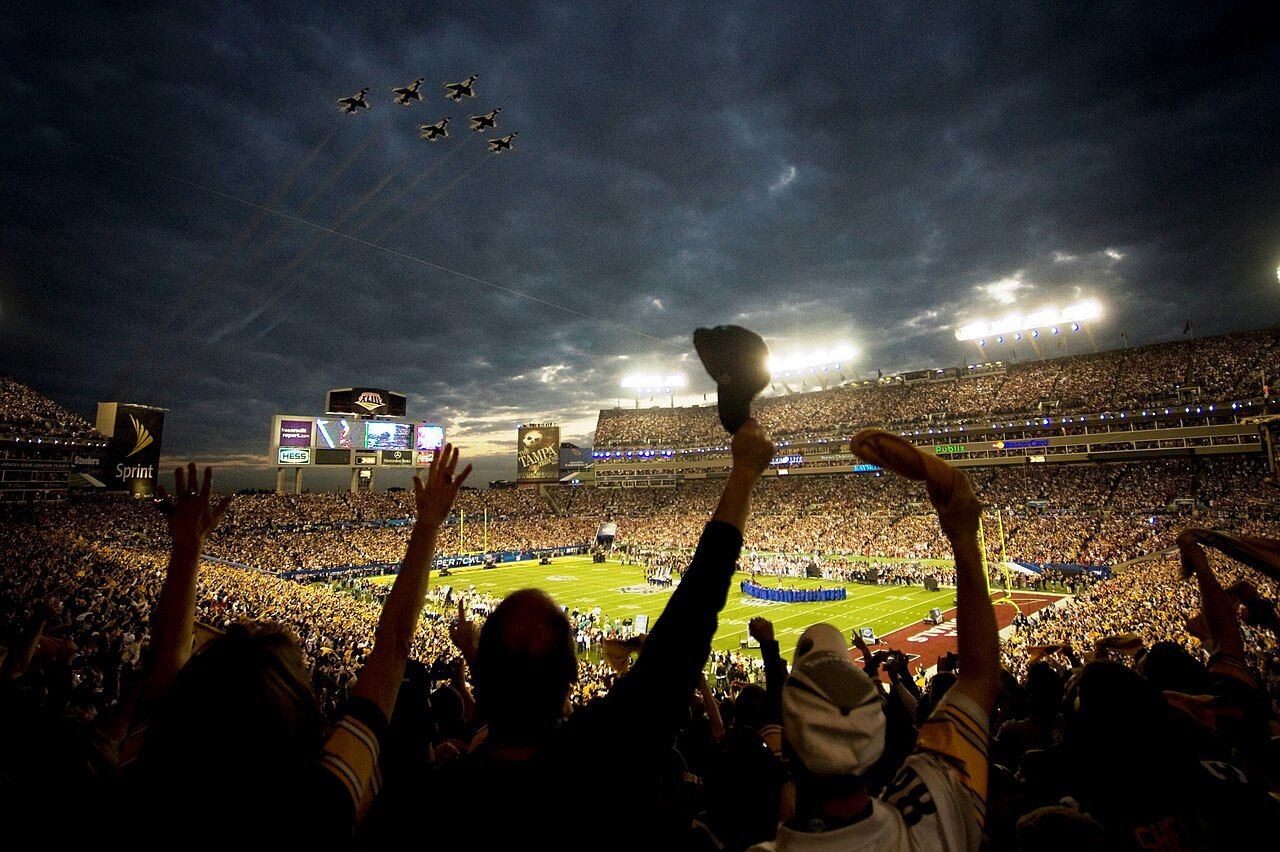
\includegraphics[width=\linewidth]{superbowl.jpg}
      \credit{Super Bowl XLIII, 2009. US Air Force, public domain}
    \end{column}
  \end{columns}
  \source{Sources: Nielsen; National Chicken Council (2026).}
\end{frame}

% ===================== Round 2 =====================
\round{2}{Super Bowl 2026}{TV viewers in the USA}{125.6\unit{million}}
  {Thanksgiving}{Turkeys eaten in one day}{$\approx$\,30\unit{million}}{LOWER}
  {Source: National Turkey Federation (estimate for Thanksgiving 2025).}

\begin{frame}{Thanksgiving}
  \begin{columns}[c]
    \begin{column}{0.55\textwidth}
      \begin{itemize}\setlength{\itemsep}{0.55em}
        \item Fourth Thursday in November: this year, \alert{November 26}
        \item 1621: Pilgrims and Wampanoag share a harvest meal
        \item A national holiday since 1863 (Abraham Lincoln)
        \item Turkey, stuffing, cranberry sauce, pumpkin pie
        \item The President ``pardons'' a turkey every year
        \item The next day is Black Friday
      \end{itemize}
    \end{column}
    \begin{column}{0.4\textwidth}
      \centering
      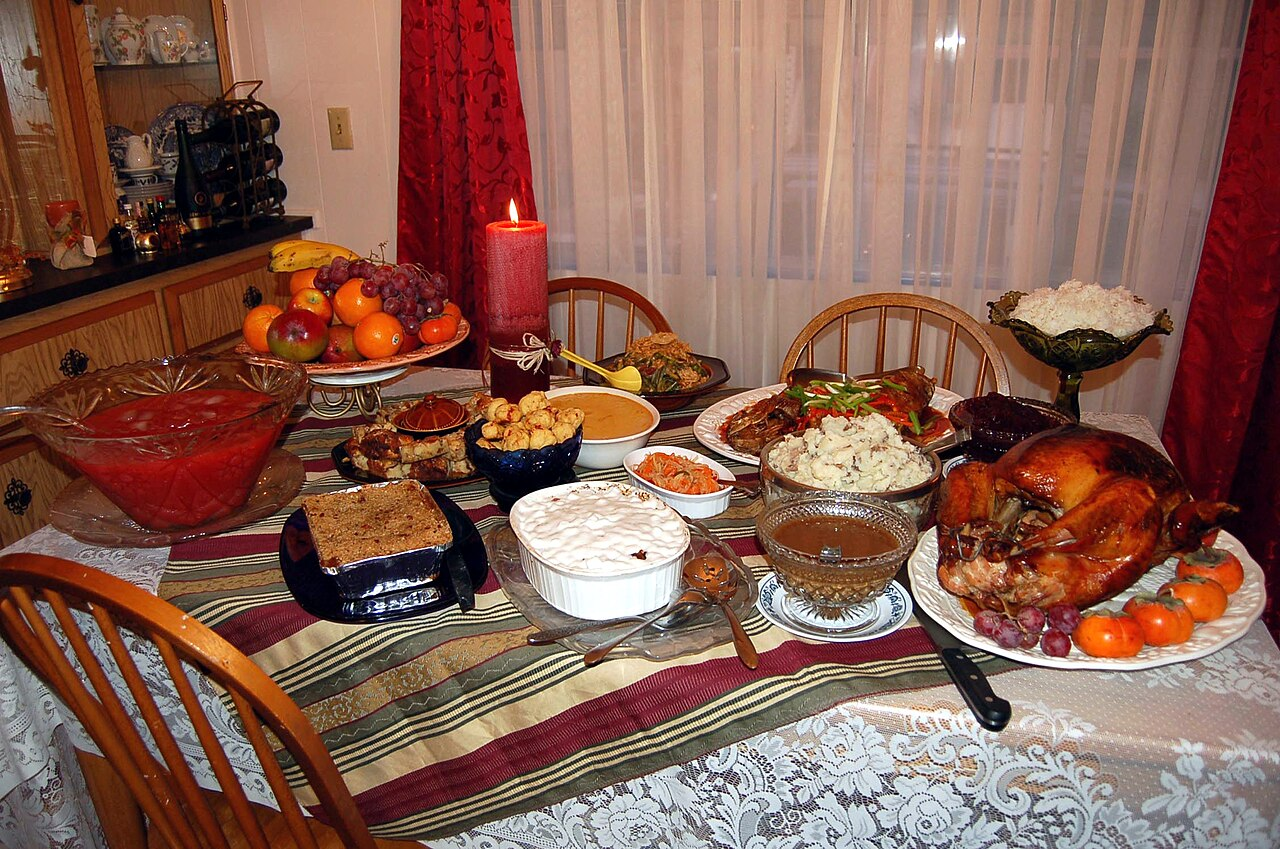
\includegraphics[width=\linewidth]{dinner.jpg}
      \credit{Photo: Ms Jones, CC BY 2.0}
    \end{column}
  \end{columns}
\end{frame}

% ===================== Round 3 =====================
\round{3}{Thanksgiving}{Turkeys eaten in one day}{$\approx$\,30\unit{million}}
  {Fourth of July}{Hot dogs eaten in one day}{150\unit{million}}{HIGHER}
  {Source: National Hot Dog and Sausage Council (industry estimate).}

\begin{frame}{The Fourth of July}
  \begin{columns}[c]
    \begin{column}{0.55\textwidth}
      \begin{itemize}\setlength{\itemsep}{0.55em}
        \item Independence Day: the Declaration of Independence, July 4, 1776
        \item 2026 was the USA's \alert{250th birthday}
        \item Barbecues, parades, fireworks
        \item Nathan's Hot Dog Eating Contest, Coney Island, New York
        \item 2026 winner: Joey Chestnut, \alert{66 hot dogs in 10 minutes}
        \item His record is 76
      \end{itemize}
    \end{column}
    \begin{column}{0.4\textwidth}
      \centering
      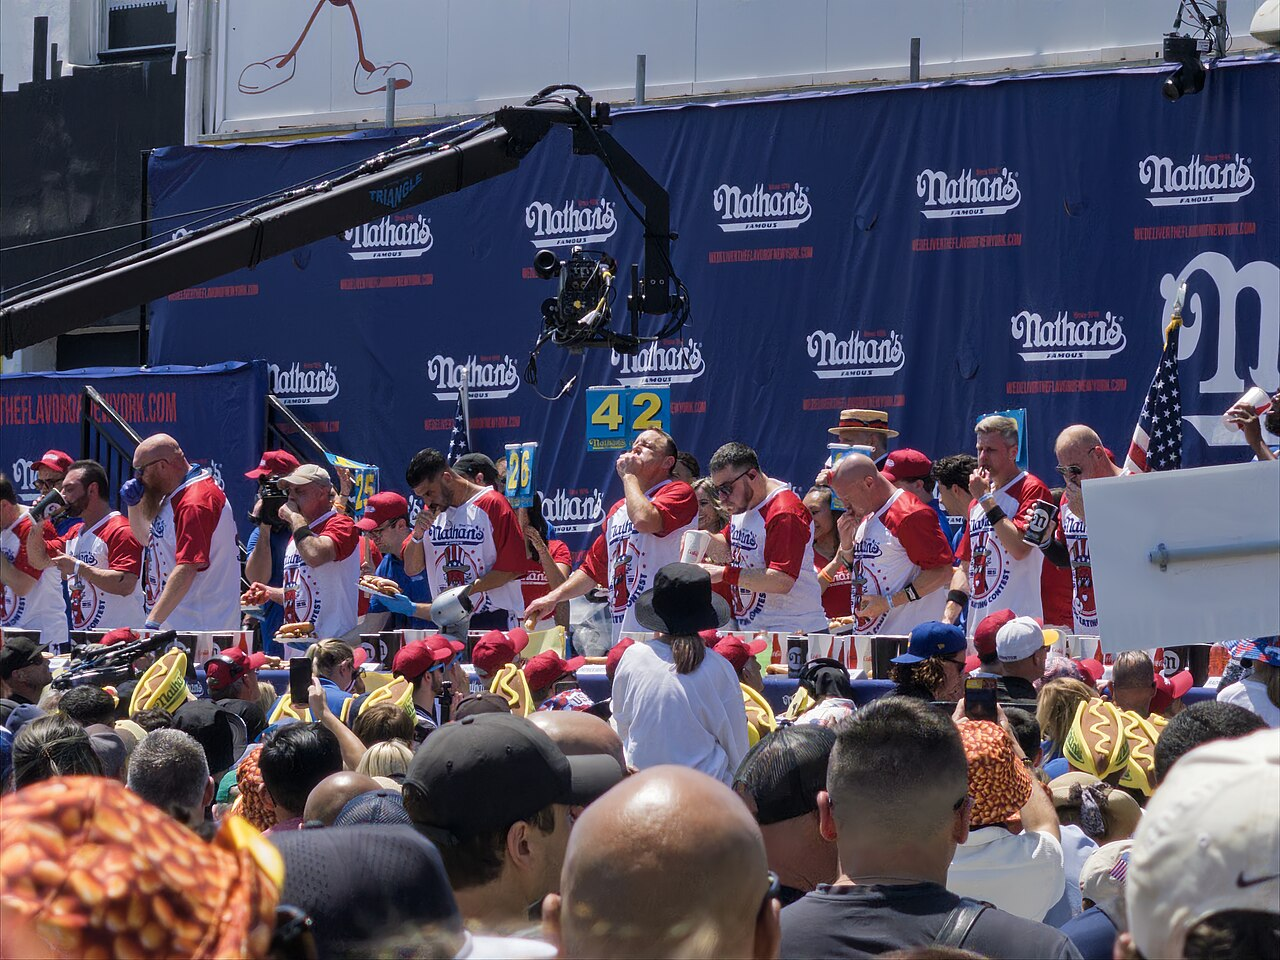
\includegraphics[width=\linewidth]{chestnut.jpg}
      \credit{Nathan's contest, 2025. Photo: SOCJ, CC BY 4.0}
    \end{column}
  \end{columns}
  \source{Source: AP (July 4, 2026).}
\end{frame}

% ===================== Round 4 =====================
\round{4}{Fourth of July}{Hot dogs eaten in one day}{150\unit{million}}
  {Bruno Mars}{Monthly listeners on Spotify}{$\approx$\,125\unit{million}}{LOWER}
  {Source: Spotify via kworb.net (November 10, 2026).}

\begin{frame}{Bruno Mars}
  \begin{columns}[c]
    \begin{column}{0.6\textwidth}
      \begin{itemize}\setlength{\itemsep}{0.55em}
        \item Born 1985 in Honolulu, Hawaii
        \item The \alert{most-listened-to} artist on Spotify
        \item First artist ever to pass 150 million monthly listeners (2025)
        \item Played the Super Bowl halftime show in 2014
        \item ``Uptown Funk'', ``Die With a Smile'' (with Lady Gaga), ``APT.'' (with Ros\'e)
        \item 2026: new album \emph{The Romantic} and a stadium tour
      \end{itemize}
    \end{column}
    \begin{column}{0.33\textwidth}
      \centering
      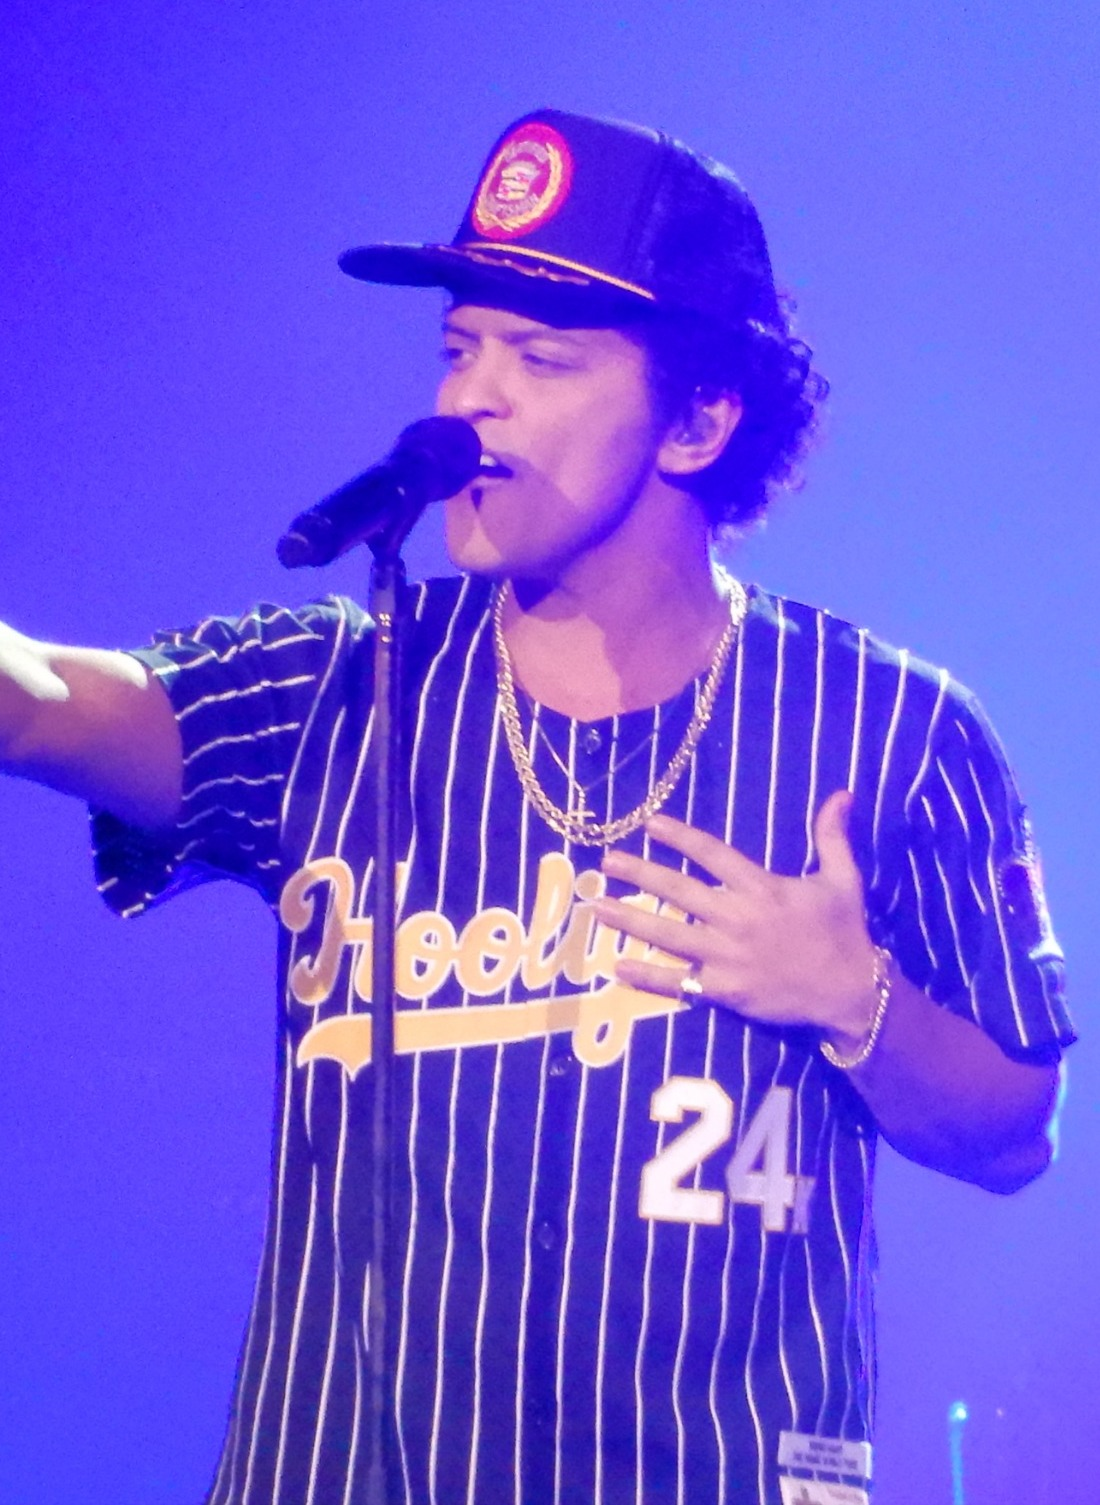
\includegraphics[height=5.2cm]{mars.jpg}
      \credit{2017. Photo: slgckgc, CC BY 4.0}
    \end{column}
  \end{columns}
  \source{Sources: Guinness World Records (2025); Atlantic Records (2026).}
\end{frame}

% ===================== Round 5 =====================
\round{5}{Bruno Mars}{Monthly listeners on Spotify}{$\approx$\,125\unit{million}}
  {US national parks}{Visits in one year}{323\unit{million}}{HIGHER}
  {Source: National Park Service (2025 visits).}

\begin{frame}{National parks}
  \begin{columns}[c]
    \begin{column}{0.6\textwidth}
      \begin{itemize}\setlength{\itemsep}{0.55em}
        \item Yellowstone (1872) was the world's \alert{first} national park
        \item Today: 63 national parks, and more than 400 protected sites
        \item 323 million visits in 2025: almost one for every American
        \item Most visited national park: Great Smoky Mountains (11.5 million)
        \item The classic American holiday: the \alert{road trip}
        \item Austria has 6 national parks
      \end{itemize}
    \end{column}
    \begin{column}{0.33\textwidth}
      \centering
      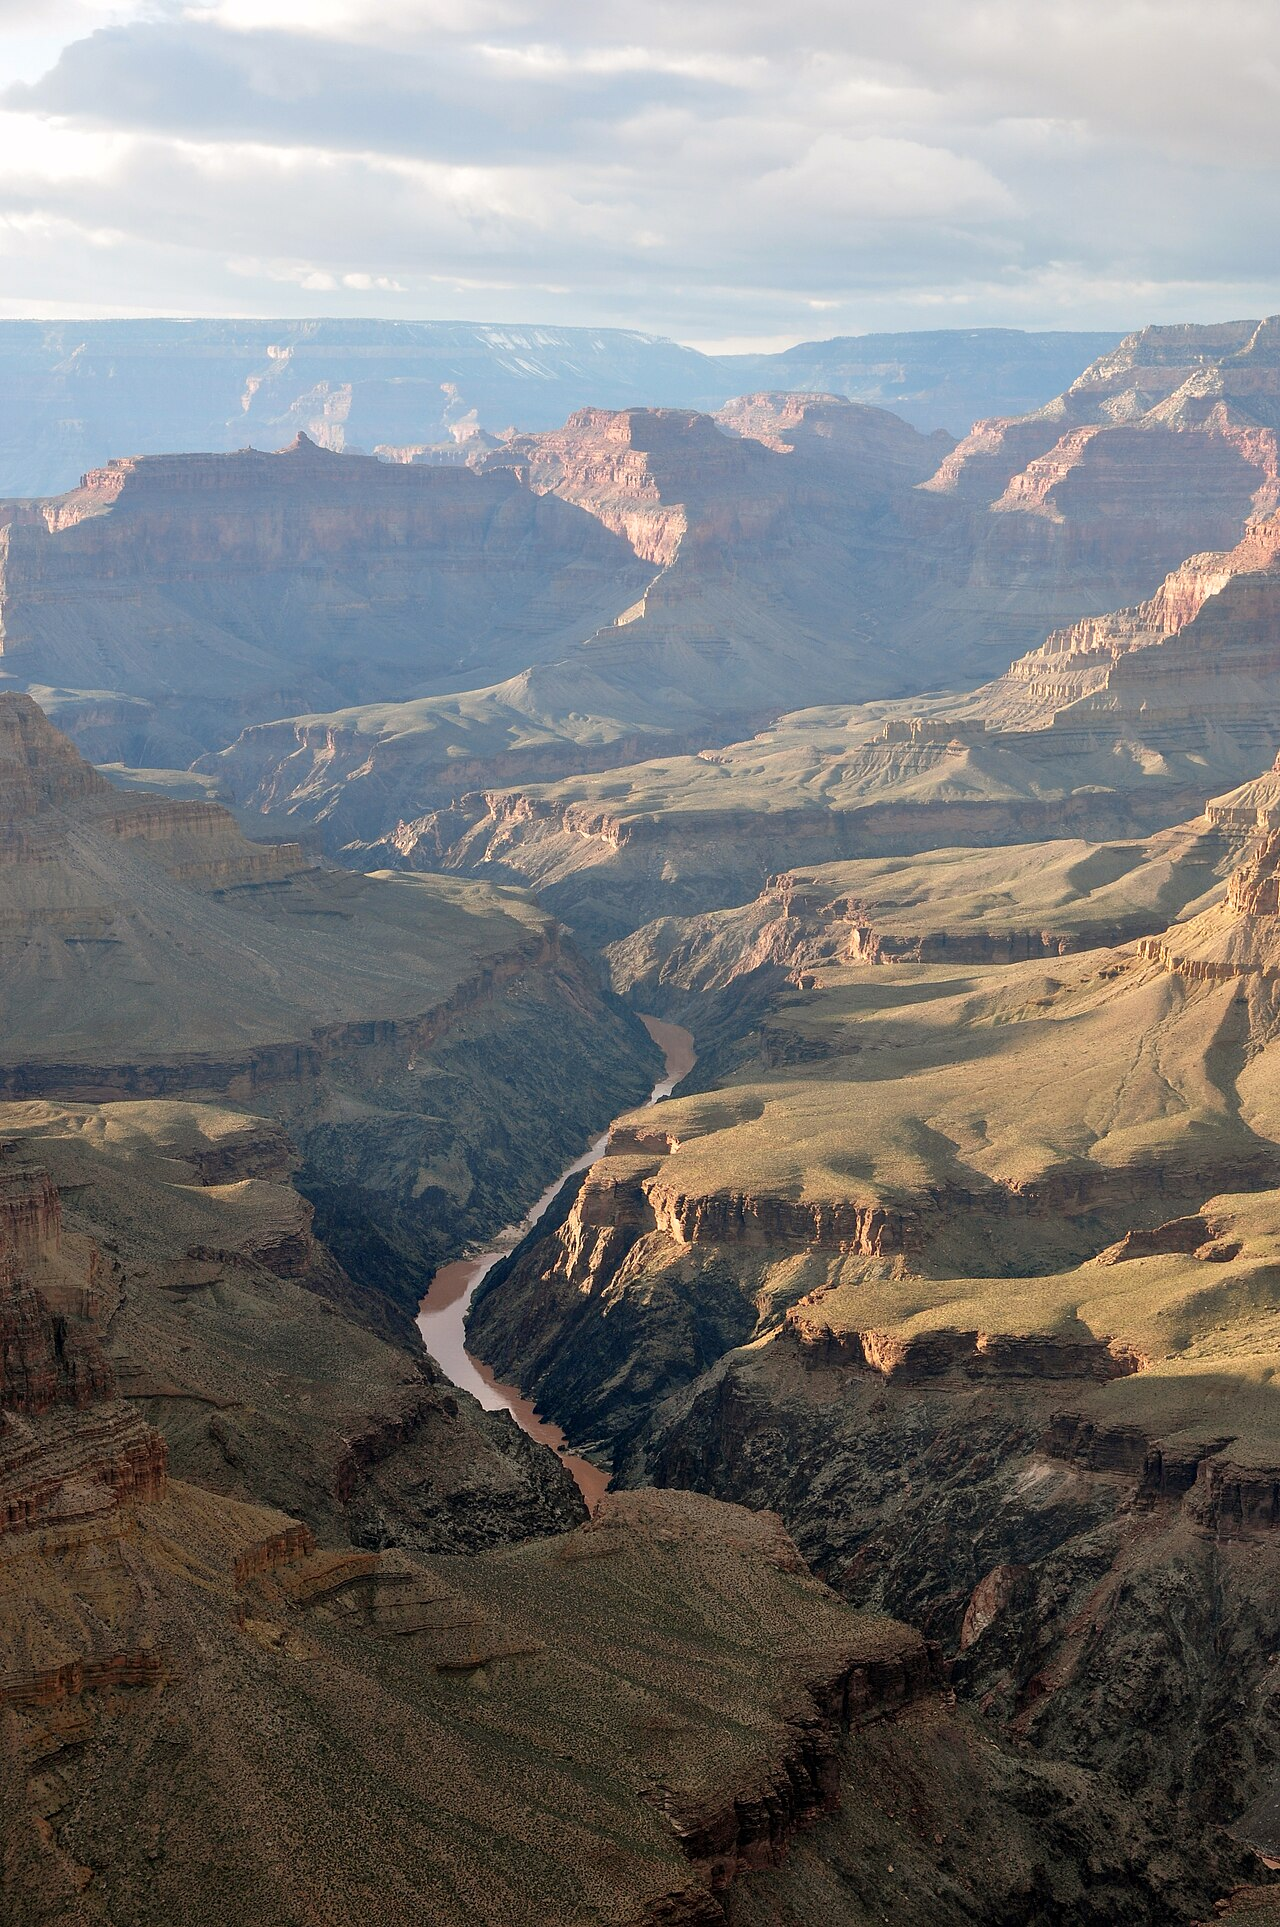
\includegraphics[height=5.2cm]{canyon.jpg}
      \credit{Grand Canyon. Photo: Chensiyuan, CC BY-SA 4.0}
    \end{column}
  \end{columns}
  \source{Source: National Park Service (2026).}
\end{frame}

% ===================== Round 6 =====================
\round{6}{US national parks}{Visits in one year}{323\unit{million}}
  {Ford F-Series pickups}{Sold in the USA in one year}{828,832\unit{trucks}}{LOWER}
  {Source: Ford (2025 sales).}

\begin{frame}{Car culture}
  \begin{columns}[c]
    \begin{column}{0.55\textwidth}
      \begin{itemize}\setlength{\itemsep}{0.55em}
        \item The best-selling vehicle in the USA is a \alert{pickup truck}
        \item The Ford F-Series has been \#1 for 44 years in a row
        \item An F-150 is almost 6 metres long
        \item Most Americans can drive alone at \alert{16}
        \item Outside a few big cities, there is no life without a car
        \item Drive-through restaurants, banks, pharmacies, even weddings
      \end{itemize}
    \end{column}
    \begin{column}{0.4\textwidth}
      \centering
      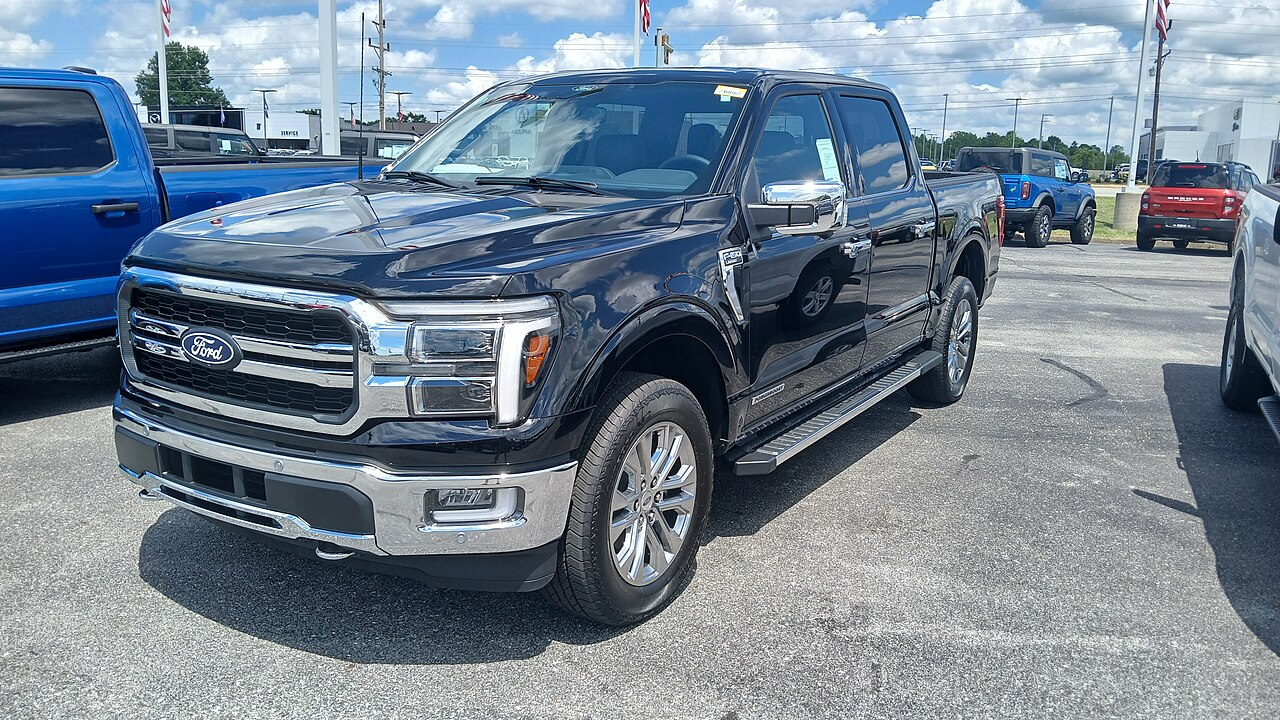
\includegraphics[width=\linewidth]{f150.jpg}
      \credit{2024 Ford F-150. Photo: Deathpallie325, CC BY 4.0}
    \end{column}
  \end{columns}
  \source{Source: Ford (2026).}
\end{frame}

% ===================== Round 7 =====================
\round{7}{Ford F-Series pickups}{Sold in the USA in one year}{828,832\unit{trucks}}
  {High school football}{Boys playing on a school team}{1,043,716\unit{players}}{HIGHER}
  {Source: NFHS High School Athletics Participation Survey (2025--26).}

\begin{frame}{School sports}
  \begin{itemize}\setlength{\itemsep}{0.15em}
    \item In the USA, sport happens at \alert{school}, not in clubs
    \item Over 8.4 million high school students play on a school team
    \item Friday night football: the whole town comes to watch
    \item Cheerleaders, marching bands, homecoming
    \item Universities too: Michigan's stadium holds \alert{107,601} people
    \item Good players can get a university scholarship
  \end{itemize}
  \centering
  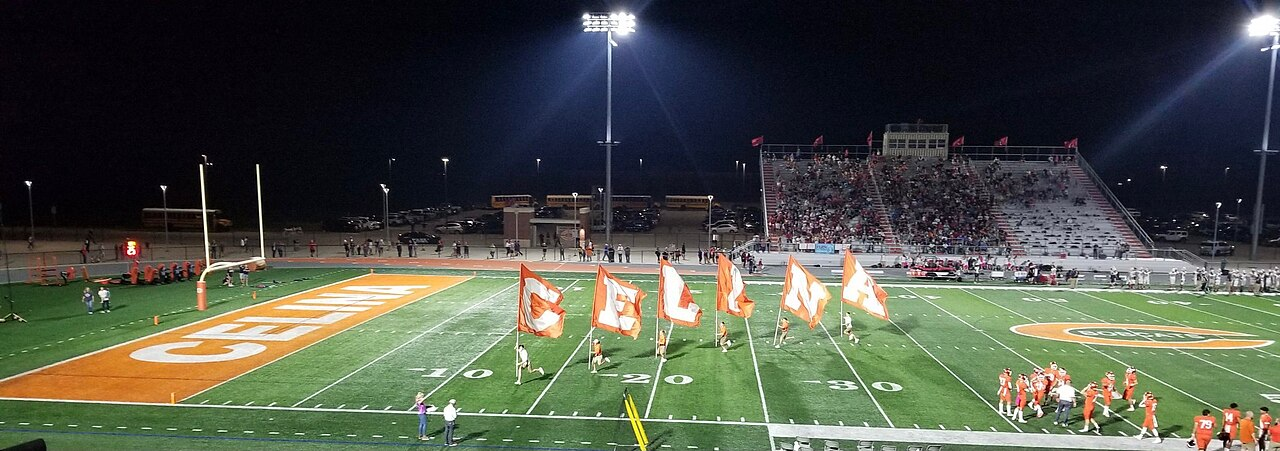
\includegraphics[width=0.5\textwidth]{football.jpg}
  \credit{Friday night football in Celina, Texas. Photo: Heidi Knapp, CC BY-SA 4.0}
  \source{Source: NFHS (2026).}
\end{frame}

% ===================== Round 8 =====================
\round{8}{High school football}{Boys playing on a school team}{1,043,716\unit{players}}
  {McDonald's}{Restaurants in the USA}{$\approx$\,13,800\unit{restaurants}}{LOWER}
  {Source: McDonald's (September 2026).}

\begin{frame}{Fast food}
  \begin{itemize}\setlength{\itemsep}{0.8em}
    \item McDonald's started in California in 1940
    \item Ray Kroc turned it into a franchise from 1955
    \item About 13,800 in the USA; about 200 in Austria
    \item About \alert{one in three} American adults eats fast food on a given day
    \item Free refills, huge portions, drive-throughs
    \item Other giants: Subway, Starbucks, Chick-fil-A, Taco Bell
  \end{itemize}
  \source{Source: CDC, National Center for Health Statistics (2021--23 data).}
\end{frame}

% ===================== Round 9 =====================
\round{9}{McDonald's}{Restaurants in the USA}{$\approx$\,13,800\unit{restaurants}}
  {One year at Harvard}{Tuition, room and food}{\$91,634\unit{dollars}}{HIGHER}
  {Source: Harvard University (cost of attendance, 2026--27).}

\begin{frame}{Paying for college}
  \begin{columns}[c]
    \begin{column}{0.55\textwidth}
      \begin{itemize}\setlength{\itemsep}{0.55em}
        \item \$91,634 is the ``sticker price'': tuition, a room and food
        \item Many students pay much less, thanks to financial aid
        \item Public universities are cheaper, but still not free
        \item About 43 million Americans have student loans
        \item Average debt: about \alert{\$40,000}
        \item In Austria: \alert{\texteuro 26.20} per semester
      \end{itemize}
    \end{column}
    \begin{column}{0.4\textwidth}
      \centering
      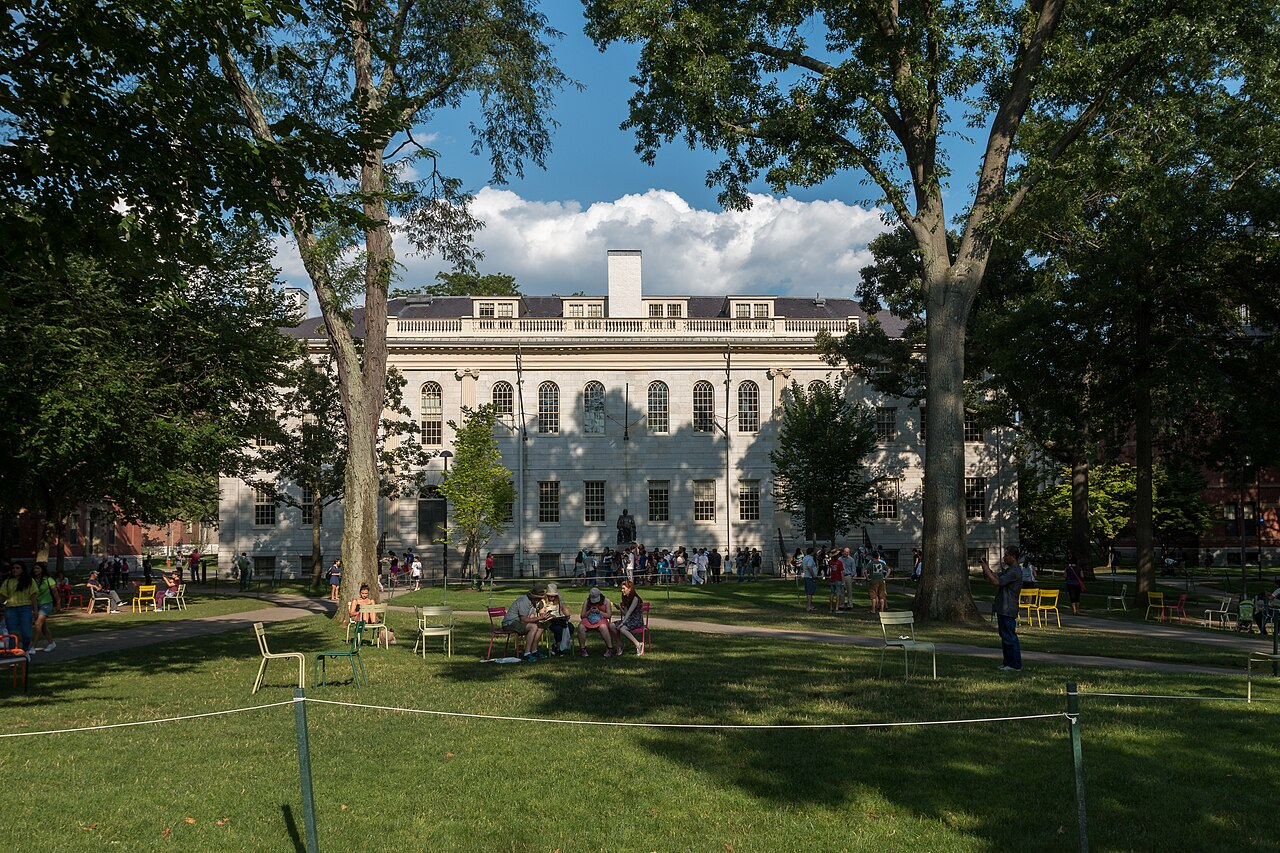
\includegraphics[width=\linewidth]{harvard.jpg}
      \credit{Harvard Yard. Photo: Marco Almbauer, public domain}
    \end{column}
  \end{columns}
  \source{Sources: Federal Student Aid; USAFacts (2026); \"OH (2026/27).}
\end{frame}

% ===================== Round 10 =====================
\round{10}{One year at Harvard}{Tuition, room and food}{\$91,634\unit{dollars}}
  {Super Bowl advert}{Price of 30 seconds}{$\approx$\,\$8\unit{million}}{HIGHER}
  {Sources: Financial Times; Wall Street Journal (2026).}

\begin{frame}{The adverts are the show}
  \begin{itemize}\setlength{\itemsep}{0.9em}
    \item \$8 million for 30 seconds: about \alert{\$267,000 per second}
    \item Many Americans watch the Super Bowl \emph{for} the adverts
    \item Companies release them online days before the game
    \item Celebrities, jokes, talking animals
    \item The same price as \alert{87 years} at Harvard
  \end{itemize}
\end{frame}

% ===================== Final score =====================
\begin{frame}{Final score}
  \renewcommand{\arraystretch}{1.7}
  \centering\large
  \begin{tabular}{@{}rl@{}}
    {\bfseries\color{oldred}10} & Honorary American \\
    {\bfseries\color{oldred}7--9} & Ready for a road trip \\
    {\bfseries\color{oldred}4--6} & Needs more hot dogs \\
    {\bfseries\color{oldred}0--3} & At least you know Eurovision \\
  \end{tabular}
\end{frame}

\begin{thinkframe}
  {\color{oldred}\textbf{Think}}\\[0.8em]
  Which number surprised you most?\\[0.6em]
  What would the Austrian version of this game look like?
\end{thinkframe}

\end{document}
